\chapter{Digital Communications}

The expression \emph{digital communications} broadly refers to the transmission of information using digital messages, or a bit stream.
There are notable advantages to transmitting data  using discrete messages.
It allows for enhanced signal processing and quality control.
In particular, errors caused by noise and interference can be detected and corrected.
Digital communications also make the networking of heterogeneous systems possible, with the Internet being the most obvious such example.
These advantages, and many more, explain the widespread adoption and constantly increasing popularity of digital communication systems.


\section{System Components}

A typical digital communication system can be represented by the functional block diagram depicted in Fig~\ref{figure:BlockDiagram}.
It is composed of five basic components.
The input block contains the source, which produces data (such as voice, emails, or images), and it also includes all the operations that are required to convert the original information into a format suitable for transmission.
The transmitter takes bits from the input block and sends them over a channel using electro-magnetic signals, or some alternate means.
Communication channels come in many flavors.
For instance, a transmission can take place over an ethernet cable, a coaxial cable, or free-space (wireless communications).
There are also more esoteric channels like a hard drive platter, a compact disc, or a memory stick.
The role of the receiver is to recover the sent message from a collection of measurements.
It may need to extract the signal from noise and, possibly, correct errors that may have occurred during transmission.
Finally, the output block takes the received information and puts it back in a format that is appropriate for the end-user.

\begin{figure}[htbp]
\begin{center}
\begin{psfrags}
\psfrag{I}[c]{Input}
\psfrag{O}[c]{Output}
\psfrag{T}[c]{Transmitter}
\psfrag{R}[c]{Receiver}
\psfrag{C}[c]{Channel}
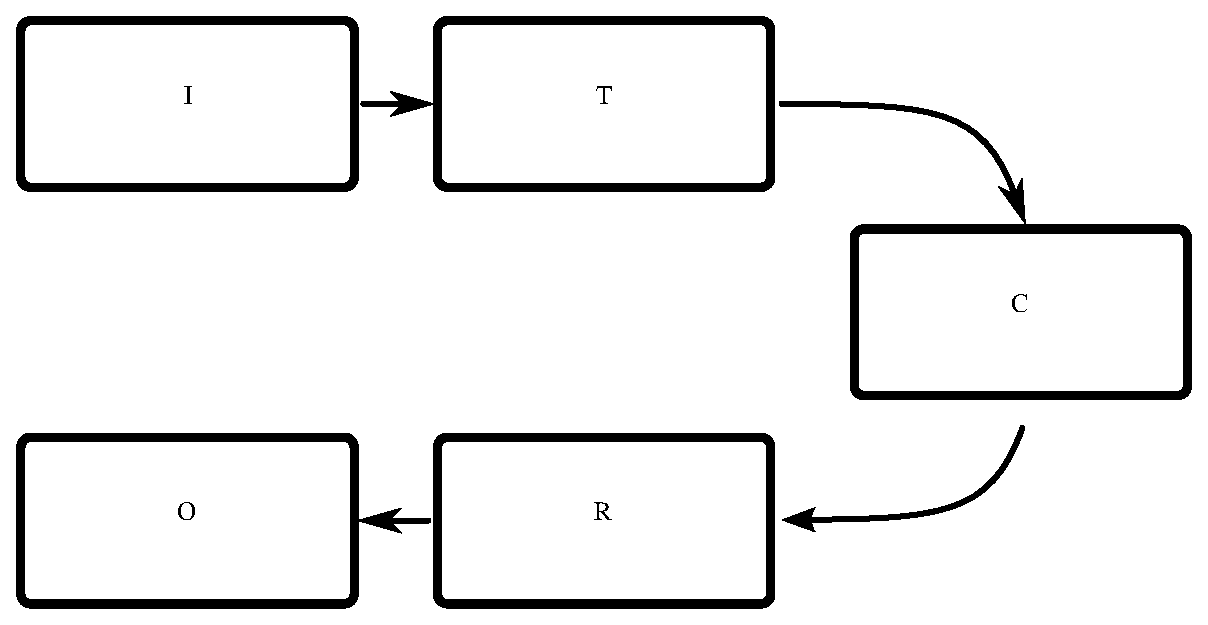
\epsfig{file=Figures/diagram,width=10.575cm}
\end{psfrags}
\end{center}
\caption{Block diagram of a digital communication system.}
\label{figure:BlockDiagram}
\end{figure}

Fig.~\ref{figure:BlockDiagram} also allude to the natural symmetry present in digital communication systems.
Operations that take place on the transmitter side must often be undone on the receiver side.
As such, complementary steps are frequently studied in pairs.
Our treatment of digital communications will follow this general approach.


\subsection{The Input-Output Blocks}

\begin{figure}[htbp]
\begin{center}
\begin{psfrags}
\psfrag{I}[c]{Input}
\psfrag{S}[c]{Sampling}
\psfrag{Q}[c]{Quantization}
\psfrag{E}[c]{Compression}
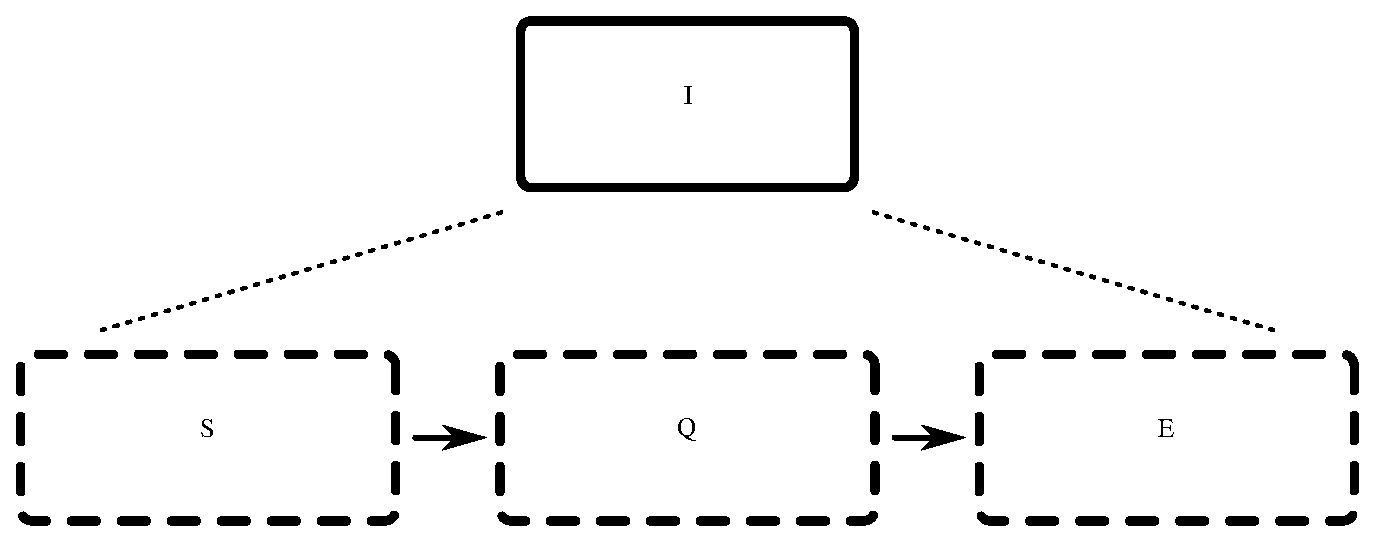
\epsfig{file=Figures/input,width=12.075cm}
\end{psfrags}
\end{center}
\caption{Components of the input block.}
\label{figure:BlockInput}
\end{figure}

\begin{figure}[htbp]
\begin{center}
\begin{psfrags}
\psfrag{O}[c]{Output}
\psfrag{I}[c]{Interpolation}
\psfrag{D}[c]{Decompression}
\epsfig{file=Figures/output,width=12.075cm}
\end{psfrags}
\end{center}
\caption{Components of the output block.}
\label{figure:BlockOutput}
\end{figure}


\subsection{The Transmitter-Receiver Pair}

\begin{figure}[htbp]
\begin{center}
\begin{psfrags}
\psfrag{T}[c]{Transmitter}
\psfrag{E}[c]{Encoder}
\psfrag{M}[c]{Modulation}
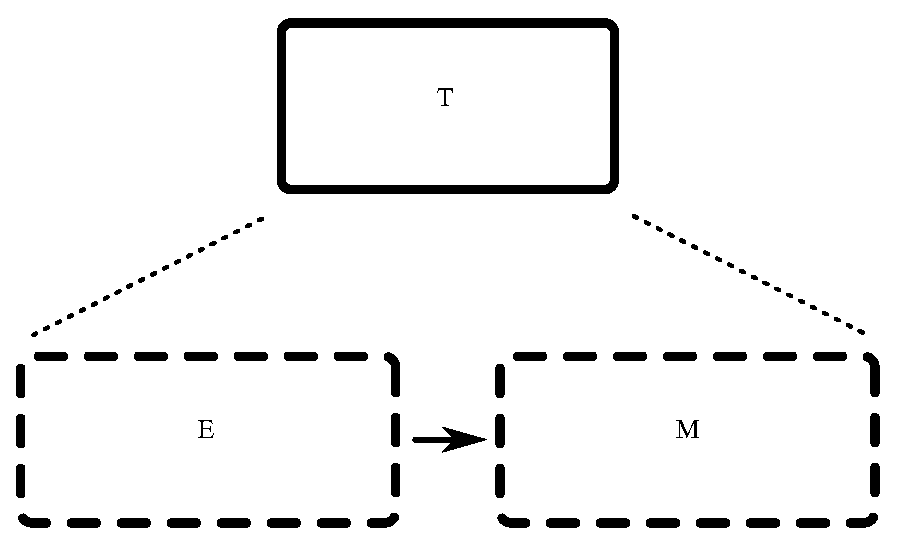
\epsfig{file=Figures/transmitter,width=7.7625cm}
\end{psfrags}
\end{center}
\caption{Components of a tranmtter.}
\label{figure:BlockTransmitter}
\end{figure}

\begin{figure}[htbp]
\begin{center}
\begin{psfrags}
\psfrag{R}[c]{Receiver}
\psfrag{M}[c]{Demodulation}
\psfrag{D}[c]{Decoder}
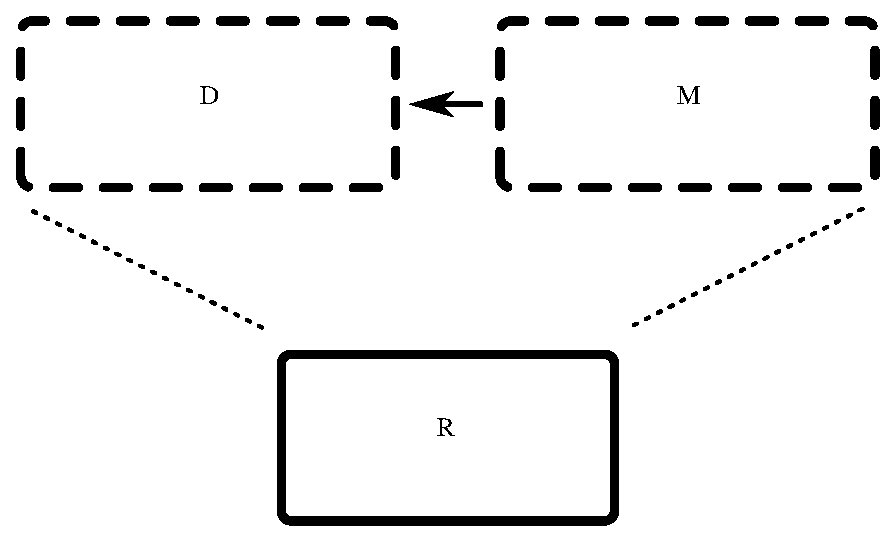
\epsfig{file=Figures/receiver,width=7.7625cm}
\end{psfrags}
\end{center}
\caption{Components of a receiver.}
\label{figure:BlockReceiver}
\end{figure}


\section{Common Channels}


\section{Sample Applications}

Digital communication occupies a central role in almost every aspect of contemporary life.
Most businesses rely on networked computers and the Internet for day-to-day operations, and digital technologies play a central role in the entertainment industry today.
Below, we provide a few examples of digital communication systems that you may be familiar with.

\paragraph{Cable Modem:}
A cable modem enables point-to-point communication over the cable television infrastructure.
They are primarily employed to deliver broadband Internet access, taking advantage of unused bandwidth on a cable television network.
With the advent of Voice over IP telephony, cable modems can also be used to provide telephone service.

\paragraph{Wi-Fi Technology:}
Wi-Fi is a global set of standards that allows wireless inter-networking.
In particular, it includes the IEEE 802.11 protocol suite (e.g., 802.11b, 802.11g, and 802.11n).
Wireless access points, also called \emph{hotspots}, often provide users with access the Internet.
Wi-Fi products can be used as an enabling technology for \emph{mesh networks}, which offer connectivity to large urban communities.

\paragraph{Bluetooth:}
Bluetooth is a wireless protocol designed for short-range communication, and it is used primarily to create personal area networks.
Bluetooth provides a means to exchange information between such devices such as mobile phones, personal computers, digital cameras, and a myriad of accessories.

\paragraph{Hard Disk Drive:}
A hard disk drive is a non-volatile storage device that stores digitally encoded data on rapidly rotating platters with magnetic surfaces.
Today, hard drives can be found in computers, digital audio players, personal digital assistants, game consoles and other embedded computing devices.
Data on a hard disk drive is recorded by magnetizing ferromagnetic material directionally, and is read back by detection the magnetization of the material.

\paragraph{Compact Disc:}
The compact disc (CD) is an optical disc used to store digital data, and remains one of the popular playback media for commercial audio recordings.
A standard compact disc can store approximately 650 Megabytes of data.
In a recordable compact disc (CD-R), a photosensitive dye is used.
The write laser of a CD recorder changes the color of the dye to allow a standard CD player to read the data, just as it would with a standard stamped disc.
A re-recordable disc medium (CD-RW) uses a metallic alloy instead of a dye.
The write laser in this case is used to heat and alter the properties of the alloy, and hence change its reflectivity.
A CD-RW does not possess as great a difference in reflectivity as a stamped compact disc, and so many earlier audio players cannot read CD-RW discs, although most later CD audio players and stand-alone DVD players can. 


